\documentclass[12pt]{report}
\usepackage[pdftex]{graphicx}
\usepackage{url}
\newcommand{\HRule}{\rule{\linewidth}{0.5mm}}
% correct bad hyphenation here
\hyphenation{op-tical net-works semi-conduc-tor auto-nomous}


\begin{document}
%
% paper title
% can use linebreaks \\ within to get better formatting as desired
\title{Design of an Attitude and Heading Reference Sensor}
\author{Patrick Hickey\\pat@moreproductive.org}
\begin{titlepage}
\begin{center}

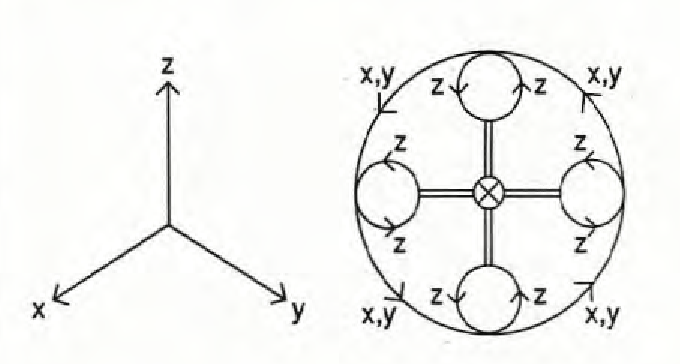
\includegraphics[width=0.3\textwidth]{./cycloid.png}\\[2cm]
\HRule \\[1cm]
{ \huge \bfseries Design of an Attitude and Heading Reference Sensor } \\[1cm]
\HRule \\[0.5cm]
{ \large \bfseries Presented for completion of an Independent Study in Electrical Engineering }
\\[0.5cm]
{ \large \bfseries Rutgers, The State University of New Jersey }
\\[0.5cm]
\HRule \\[1cm]

{\large Pat Hickey}
\\ 
pat@moreproductive.org
\\[0.5cm]
\emph{Advisor}
\\ Dr. Chung-chieh Shan
\\ Department of Computer Science
\vfill
{\large \today}

\end{center}
\end{titlepage}


\begin{abstract}
This paper describes the design of an Attitude and Heading Reference Sensor (AHRS), which measures rootational orientation relative to north and down. 
The design uses 3-axis accellerometer, magnetometer, and rate gyro sensors. 
I will discuss the selection and construction of the sensor hardware, design and implementation of a Kalman filter for sensor fusion, and the test of both the sensor hardware and software.
\end{abstract}


\section{Problem Description}

I needed to build sensor hardware and software that would determine the angular orientation and angular rotation rate of the sensor relative to the earth frame, ie. North, East, and Down. I selected sensor integrated circuits (ICs) which determine, on three axes, body accelleration, body rotation rate, and relative magnetic field. These three sensors (accellerometer, rate gyro, and magnetometer) provide a total of nine measurments. 

An algorithm is required to convert these nine measurments into an expression of angular orientation and angular rate (the derivative, with respect to time, of angular orientation). Angular orientation of a body has three degrees of freedom, as does angular rate. The conversion from measurment space to estimate space (a pair of angular orientation estimate and angular rate estimate) is nonlinear and uses a four-dimensional vector called a quaternion to describe the three-dimensional angular orientation. This is to say, a big part of the problem is ensuring the correctness of this difficult conversion process.   

I selected a well-known algorithm which implements a Quaternion Kalman Filter. This provides an state estimate using the four-dimensional quaternion vector, and an additional three-dimensional rotational rate vector. I needed to implement that software so that I could test it for correctness and use it to determine the orientation of an actual sensor. This software was to be used in an actual model aircraft autopilot system, so it must meet requirments for reliability and soft real-time performance.

\subsection{Application}

As part of my role on the Rutgers Autonomous Aircraft Team, I've been working on a model aircraft autopilot system based on a single board computer which runs Linux \footnote{For more information on this project, see \url{http://moreproductive.org/autopilot/}}. I implemented the control, navigation, and telemetry software in C using standard Linux system calls and threads. I used dedicated hardware for real-time tasks, for example, a microcontroller-based servo controller connected via USB ensures proper servo control despite irregular communication intervals from the computer. 
By using helper threads for input and output, we can be reasonably sure the main control loop will run at close to 60Hz. This is considered ``soft'' real-time.

The sensor software needs to cooperate with the soft real-time main control loop. 



aircraft autopilot
- in particular, paparazzi for linux
- soft real-time
- threads, c, linux
\subsection{Use of Haskell}
It is well established how to implement such a filter in C

I approached using a functional language as an experiment

\section{Hardware}
\subsection{Sensors}
needed 3 axis magnetometer, accellerometer, rate gyro
selected two ics:
invensense itg3200
st micro ...
\subsection{Microcontroller}
uart required to talk to a pc (ttyUSB), i2c required to talk to sensors
arduino pro mini was a simple solution, easy to use programming environment
\subsection{Construction}
provide photographs, schematic


\section{Embedded Software}
\subsection{Requirments}
timing and communication requirments of embedded hardware
st acc self test
\subsection{Communication Protocol}
serial strings etc.
\subsection{Arduino Environment}
describe arduino programming environment
blocking serial calls
-- Provide timing information?

\section{Filtration Software}
The filtration software was implemented in Haskell. The code may be found on Github at http://github.com/pchickey/hs-qkf/
\subsection{Algorithm Selection}
find an algorithm which assumes my measurment sources
\subsection{Algorithm Overview}
maybe a flow diagram would help here
\subsection{Implementation of Filter}
hmatrix-static
quaternions
\subsection{Implementation of Tests}
euler models
rotation-matrix based vector measurment simulation
addition of noise
\subsection{Sensor Interface}
serial.hs
\subsection{Gnuplot Interface}
overview, code snippets
\subsection{OpenGL Demonstration Interface}
cube.hs overview, code snippets 
\subsection{Paparazzi Autopilot Interface}
ffi, linux mq
"ongoing investigation"

\section{Results}
\subsection{Noise-free simulated measurments}
Plots of step test, ramp test
\subsection{Noisy simulated measurments}
step test, ramp test
\subsection{Tests with Sensor}
plots, link to video on youtube

\end{document}


